\clearpage
\appendix
\section{Appendix: Full Results for the Default Parameter Setup}

For completeness, all tables and figures for the default parameter setup are provided in this appendix, following the same order as the tuned setup in the main text.

\subsection{Comparison: Replication vs Paper Baselines (Extreme Traffic, Default Scenario)}

\begin{table}[H]
\centering
\small
\caption{Replication vs Paper Values (Extreme Traffic, Default Scenario)}
\begin{tabular}{l c c c}
\toprule
\textbf{Metric} & \textbf{Replication} & \textbf{Paper} & \textbf{Deviation} \\
\midrule
\multicolumn{4}{l}{\textit{ALINEA}} \\
\midrule
Throughput (veh/h)       & 4435.08 & 3790.29 & +17.01\% \\
Speed (m/s)              & 7.01    & 10.62   & $-$33.99\% \\
Stops per Vehicle        & 4.47    & 11.73   & $-$61.89\% \\
Fuel Efficiency (mpg)    & 11.64   & 16.83   & $-$30.84\% \\
CO$_2$ Emissions (g/mi)  & 836.71  & 518.52  & +61.37\% \\
NO$_x$ Emissions (mg/mi) & 357.29  & 212.66  & +68.01\% \\
\midrule
\multicolumn{4}{l}{\textit{Fixed}} \\
\midrule
Throughput (veh/h)       & 4432.57 & 3648.60 & +21.49\% \\
Speed (m/s)              & 7.05    & 9.57    & $-$26.33\% \\
Stops per Vehicle        & 4.50    & 7.18    & $-$37.33\% \\
Fuel Efficiency (mpg)    & 11.53   & 15.82   & $-$27.12\% \\
CO$_2$ Emissions (g/mi)  & 850.49  & 552.63  & +53.90\% \\
NO$_x$ Emissions (mg/mi) & 363.57  & 227.03  & +60.14\% \\
\midrule
\multicolumn{4}{l}{\textit{No Ramp Meter}} \\
\midrule
Throughput (veh/h)       & 4433.47 & 3683.02 & +20.38\% \\
Speed (m/s)              & 6.89    & 9.45    & $-$27.09\% \\
Stops per Vehicle        & 4.71    & 25.42   & $-$81.47\% \\
Fuel Efficiency (mpg)    & 11.59   & 15.25   & $-$24.00\% \\
CO$_2$ Emissions (g/mi)  & 841.01  & 575.34  & +46.18\% \\
NO$_x$ Emissions (mg/mi) & 359.21  & 236.62  & +51.81\% \\
\bottomrule
\end{tabular}
\end{table}

\subsection{Convergence Analysis of Reinforcement Learning Controllers (Default)}

\begin{figure}[H]
  \centering
  \begin{minipage}[t]{0.48\linewidth}
    \centering
    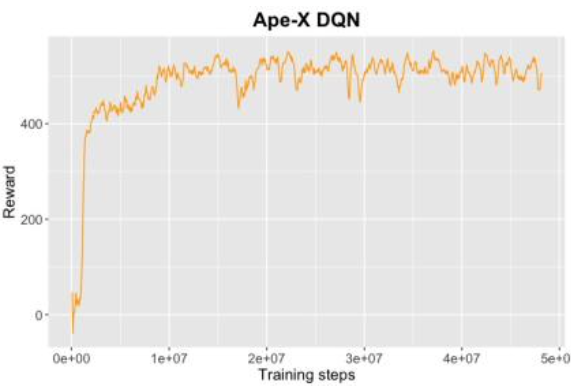
\includegraphics[width=\linewidth]{figures/results/Tuned/RL_convergence/original/apexdqn_reward.png}
  \end{minipage}
  \hfill
  \begin{minipage}[t]{0.48\linewidth}
    \centering
    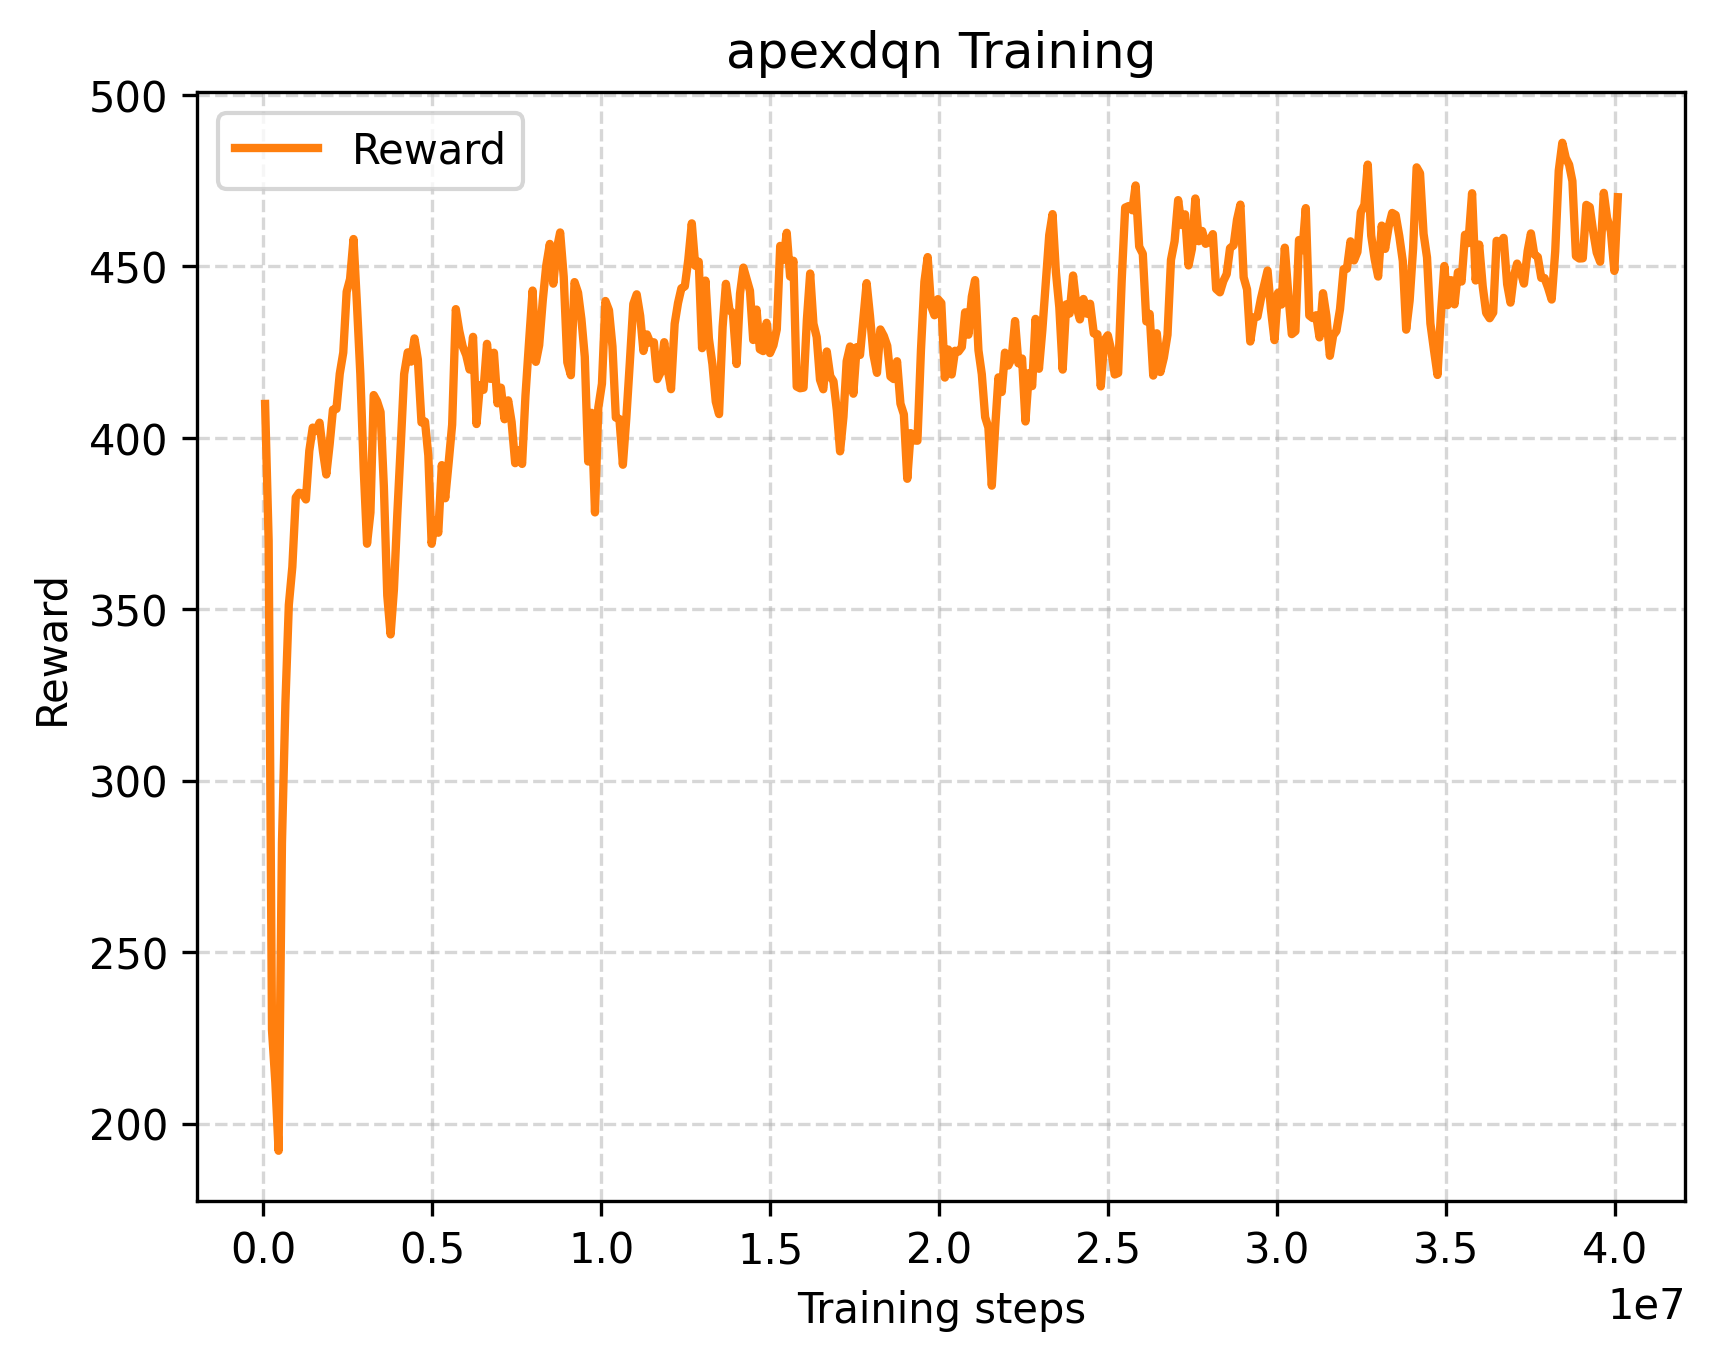
\includegraphics[width=\linewidth]{figures/results/Default/RL_convergence/apexdqn_live_reward.png}
  \end{minipage}
  \caption{Ape-X DQN training convergence (default setup): original (left) vs.\ replication (right).}
\end{figure}

\begin{figure}[H]
  \centering
  \begin{minipage}[t]{0.48\linewidth}
    \centering
    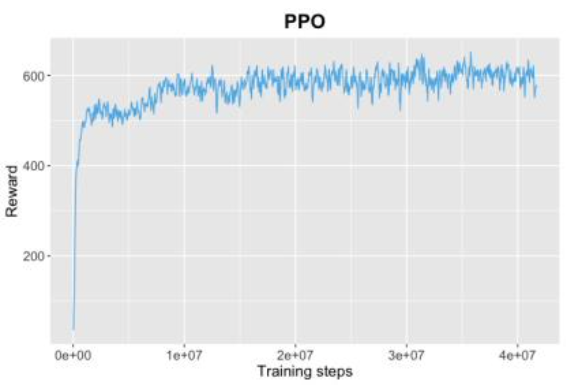
\includegraphics[width=\linewidth]{figures/results/Tuned/RL_convergence/original/ppo_reward.png}
  \end{minipage}
  \hfill
  \begin{minipage}[t]{0.48\linewidth}
    \centering
    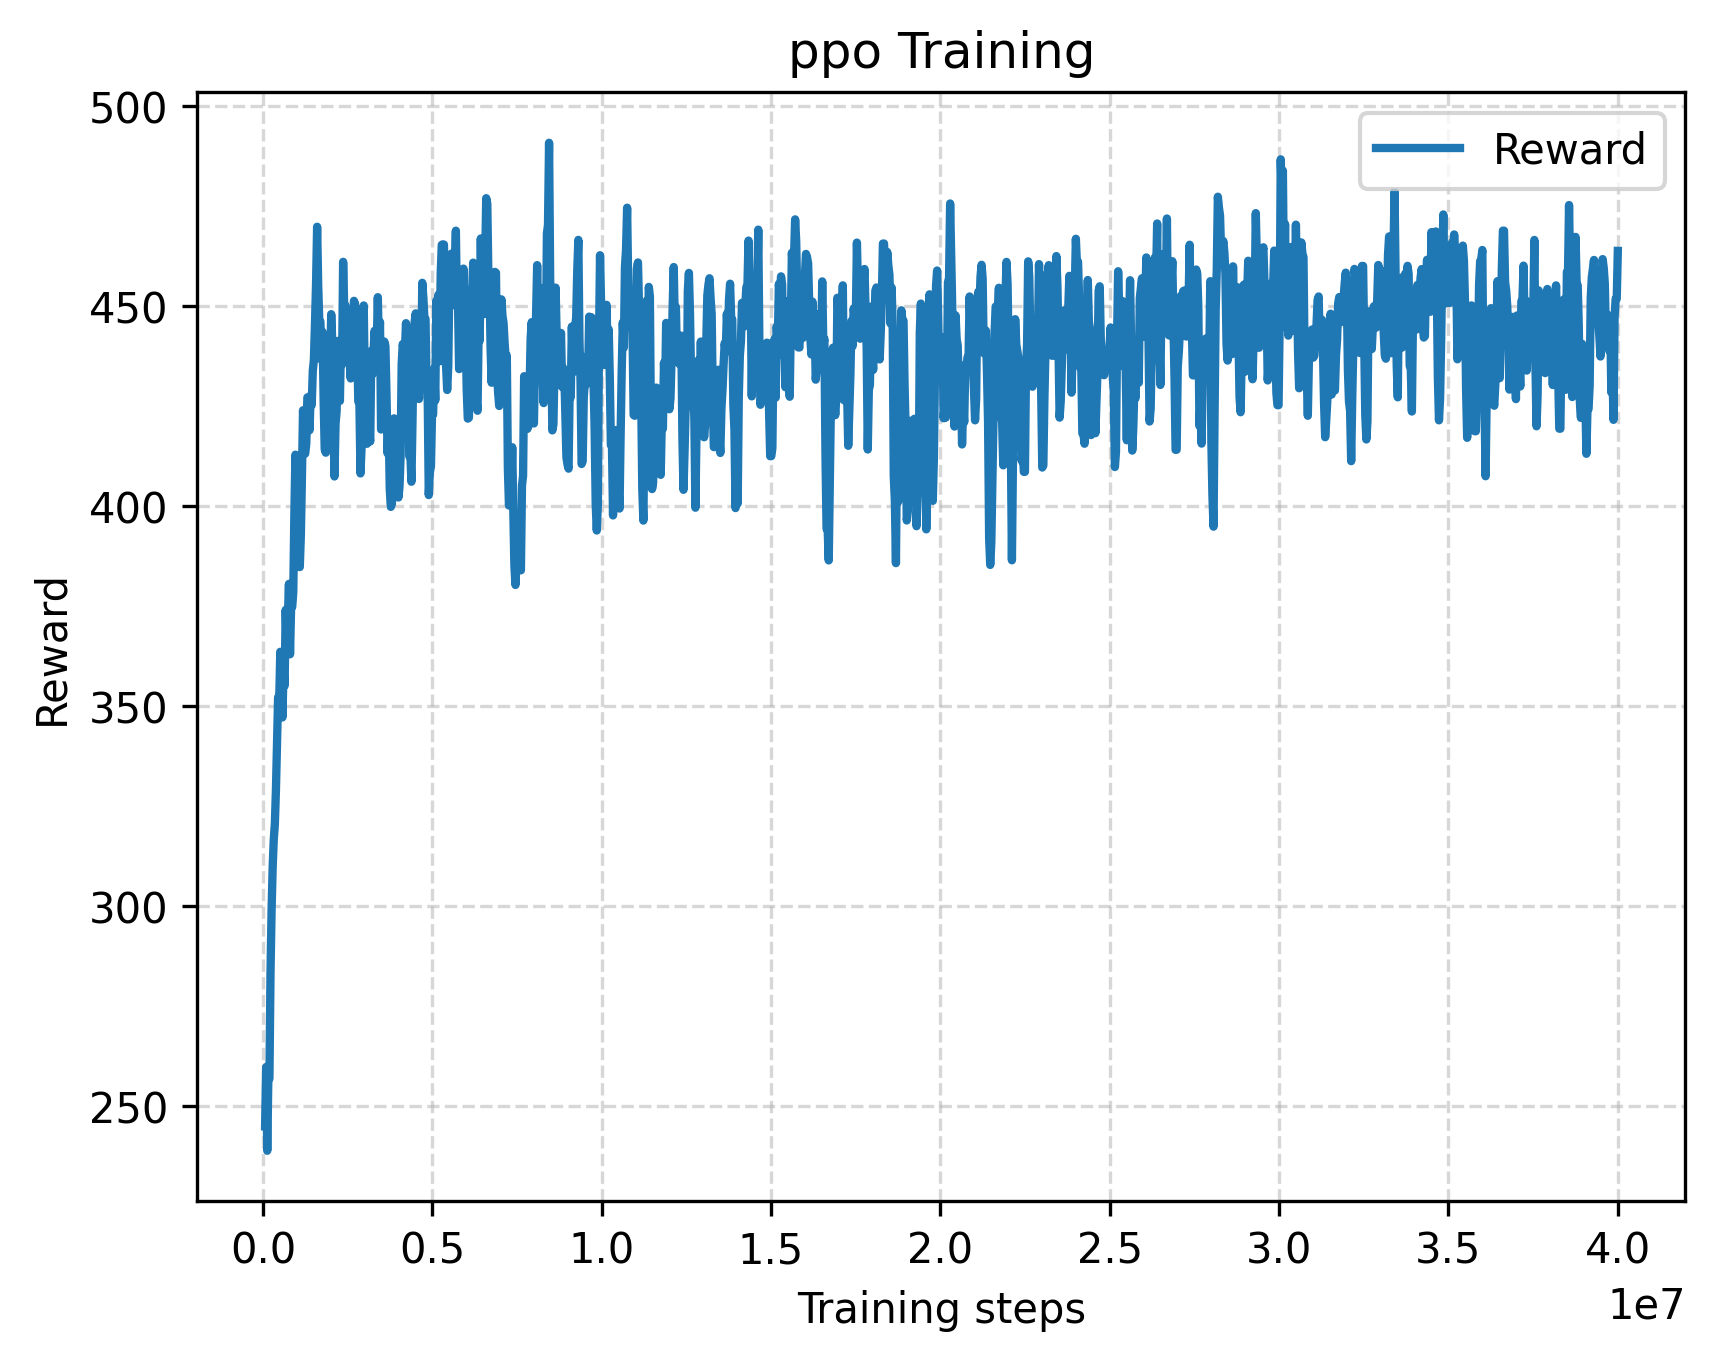
\includegraphics[width=\linewidth]{figures/results/Default/RL_convergence/ppo_live_reward.png}
  \end{minipage}
  \caption{PPO training convergence (default setup): original (left) vs.\ replication (right).}
\end{figure}

\begin{figure}[H]
  \centering
  \begin{minipage}[t]{0.48\linewidth}
    \centering
    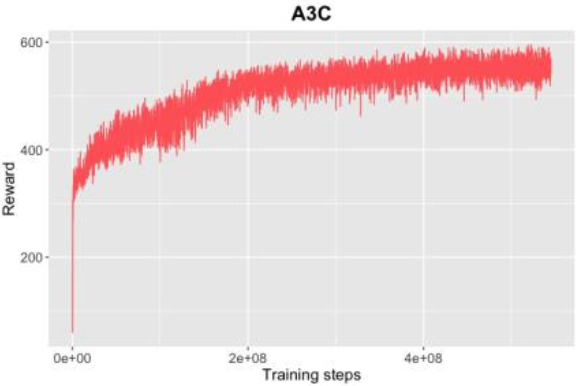
\includegraphics[width=\linewidth]{figures/results/Tuned/RL_convergence/original/a3c_reward.png}
  \end{minipage}
  \hfill
  \begin{minipage}[t]{0.48\linewidth}
    \centering
    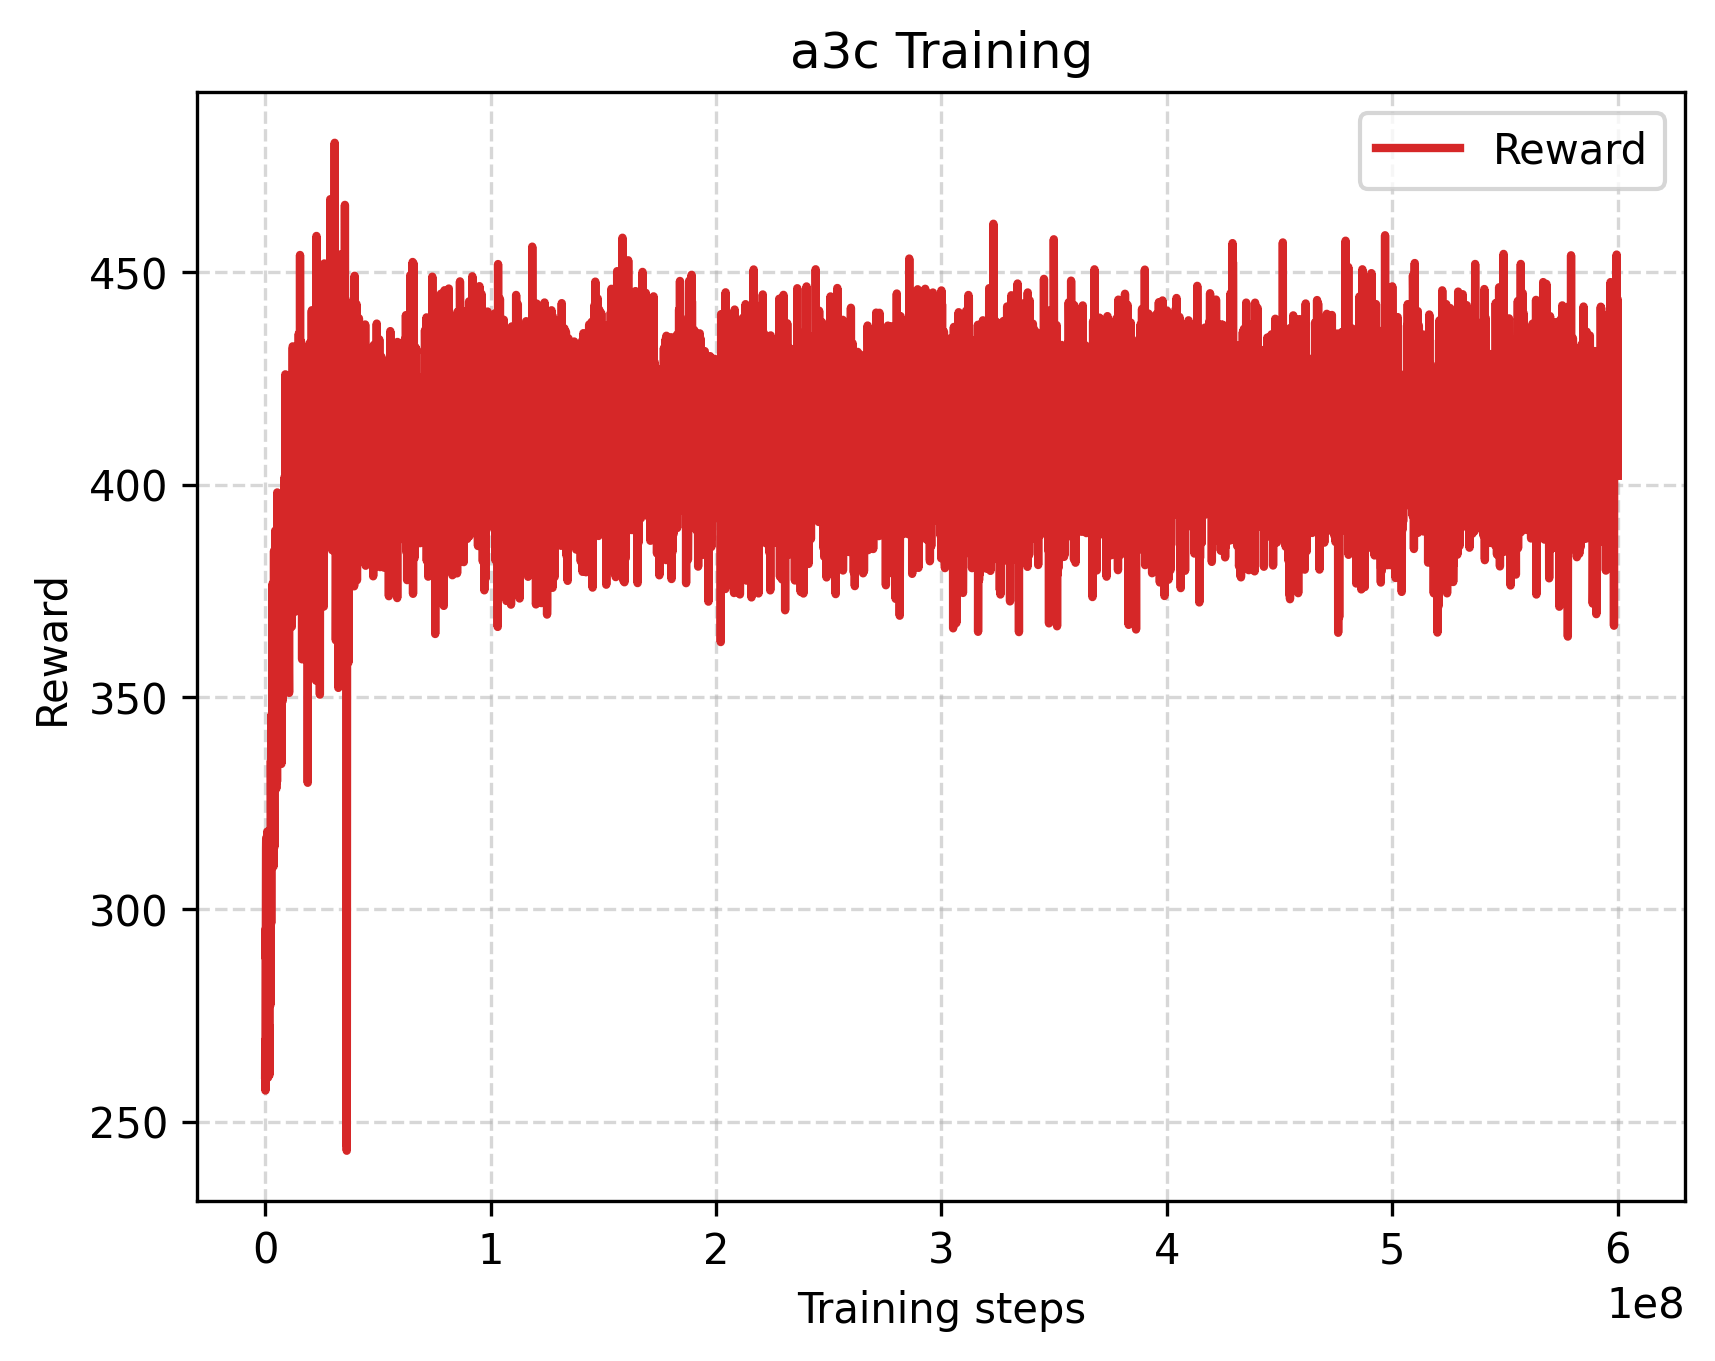
\includegraphics[width=\linewidth]{figures/results/Default/RL_convergence/a3c_live_reward.png}
  \end{minipage}
  \caption{A3C training convergence (default setup): original (left) vs.\ replication (right).}
\end{figure}

\subsection{Boxplots: RL vs Baselines (Default)}

\begin{figure}[H]
  \centering
  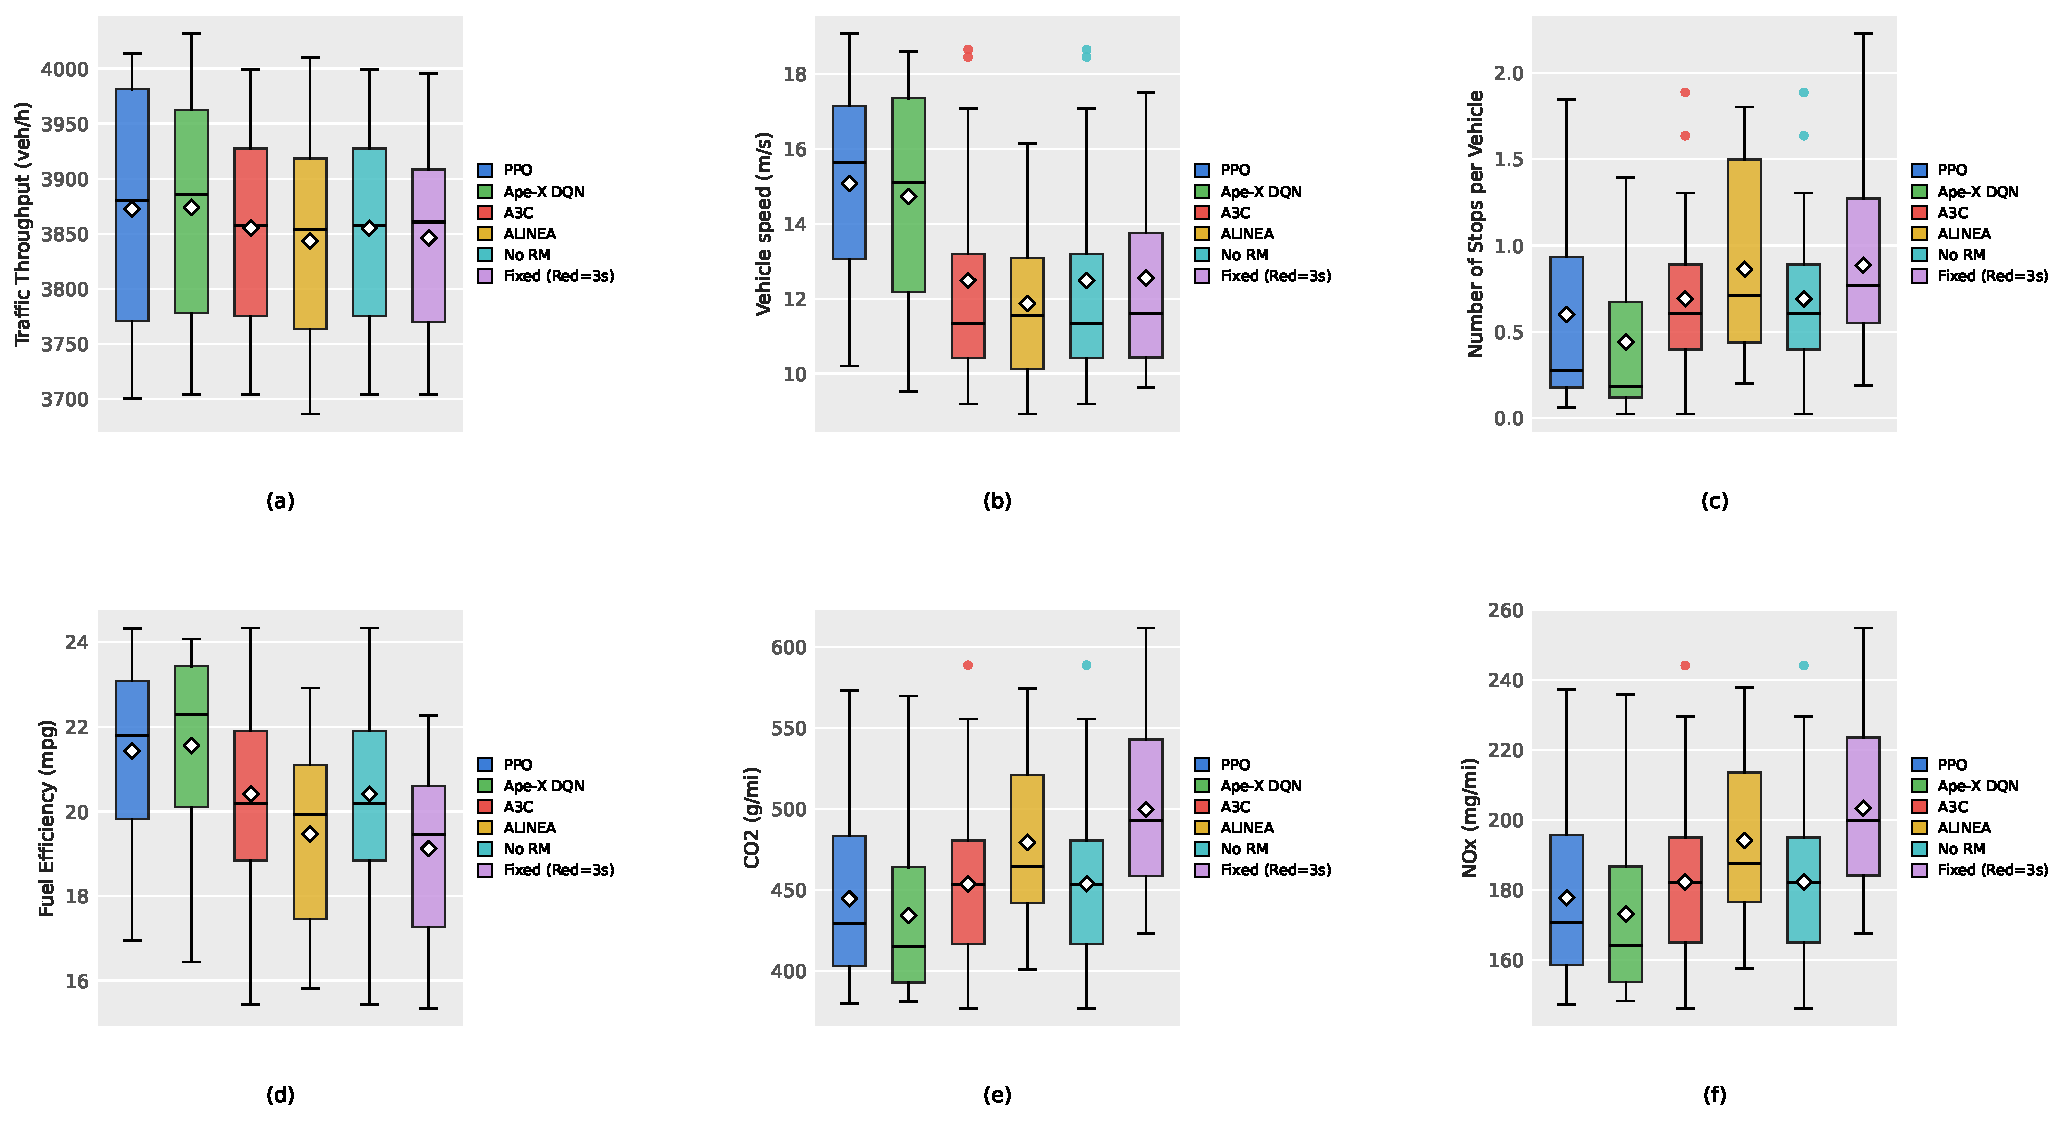
\includegraphics[width=\linewidth]{figures/results/Default/mixed/figure4_mixed.pdf}
  \caption{Performance metrics for the mixed traffic scenario (default setup). (a) Traffic Throughput (veh/h), (b) Average Vehicle Speed (m/s), (c) Number of Stops per Vehicle, (d) Fuel Efficiency (mpg), (e) CO$_2$ Emissions (g/mi), (f) NO$_x$ Emissions (mg/mi).}
\end{figure}

\begin{figure}[H]
  \centering
  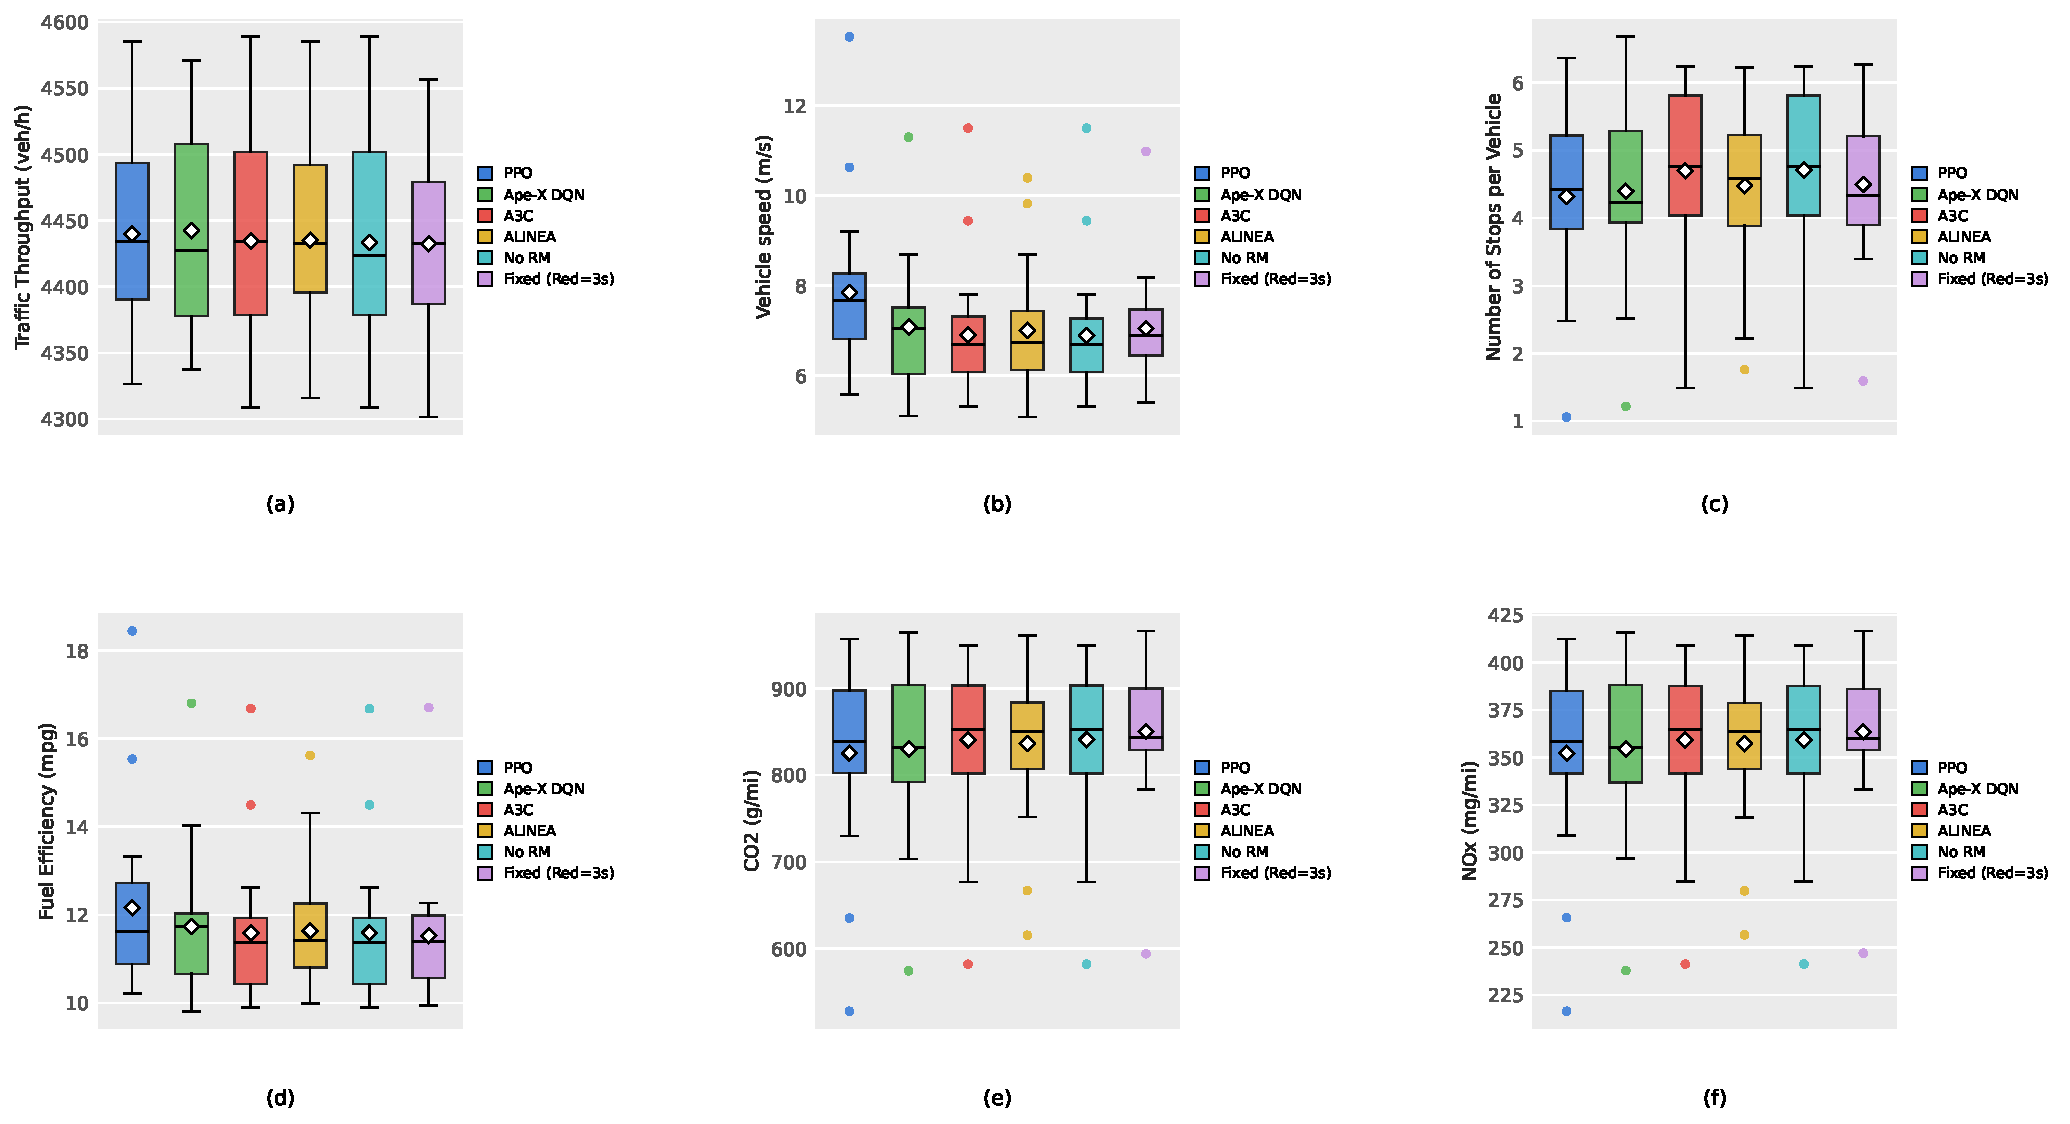
\includegraphics[width=\linewidth]{figures/results/Default/extreme/figure5_extreme.pdf}
  \caption{Performance metrics for the extreme traffic scenario (default setup). (a) Traffic Throughput (veh/h), (b) Average Vehicle Speed (m/s), (c) Number of Stops per Vehicle, (d) Fuel Efficiency (mpg), (e) CO$_2$ Emissions (g/mi), (f) NO$_x$ Emissions (mg/mi).}
\end{figure}

\subsection{Performance Comparison: RL vs Baselines (Default)}

\begin{table}[H]
\centering
\small
\caption{RL Average vs Baseline Controllers: Mixed Traffic Conditions (Default Parameters)}
\begin{tabular}{l c c c c}
\toprule
\multirow{2}{*}{\textbf{Performance Metric}} & \multirow{2}{*}{\textbf{RL Average}} & \multicolumn{3}{c}{\textbf{Changes Compared with Baseline}} \\
\cmidrule(lr){3-5}
 & & \textbf{ALINEA} & \textbf{No Ramp Meter} & \textbf{Fixed} \\
\midrule
Traffic throughput (vph)                      & 3{,}867.21 & +0.61\%  & +0.31\%  & +0.54\%  \\
Average vehicle speed (m/s)                   & 14.10      & +18.79\% & +12.89\% & +12.26\% \\
Average number of stops per vehicle           & 0.58       & $-$32.56\% & $-$15.94\% & $-$34.83\% \\
Average vehicle fuel efficiency (mpg)         & 21.13      & +8.53\%  & +3.53\%  & +10.51\% \\
Average CO$_2$ emissions per vehicle (g/mi)   & 444.40     & $-$7.33\%  & $-$2.11\%  & $-$11.09\% \\
Average NO$_x$ emissions per vehicle (mg/mi)  & 177.73     & $-$8.44\%  & $-$2.51\%  & $-$12.59\% \\
\bottomrule
\end{tabular}
\end{table}

\begin{table}[H]
\centering
\small
\caption{RL Average vs Baseline Controllers: Mixed Traffic Conditions (Original Paper)}
\begin{tabular}{l c c c c}
\toprule
\multirow{2}{*}{\textbf{Performance Metric}} & \multirow{2}{*}{\textbf{RL Average}} & \multicolumn{3}{c}{\textbf{Changes Compared with Baseline}} \\
\cmidrule(lr){3-5}
 & & \textbf{ALINEA} & \textbf{No Ramp Meter} & \textbf{Fixed} \\
\midrule
Traffic throughput (vph)                      & 3{,}738 & +2\%   & +2\%   & +7\%   \\
Average vehicle speed (m/s)                   & 19.0    & +53\%  & +72\%  & +34\%  \\
Average number of stops per vehicle           & 1.7     & $-$85\% & $-$91\% & $-$53\% \\
Average vehicle fuel efficiency (mpg)         & 22.1    & +30\%  & +38\%  & +21\%  \\
Average CO$_2$ emissions per vehicle (g/mi)   & 395     & $-$23\% & $-$28\% & $-$18\% \\
Average NO$_x$ emissions per vehicle (mg/mi)  & 156     & $-$25\% & $-$31\% & $-$20\% \\
\bottomrule
\end{tabular}
\end{table}

\begin{table}[H]
\centering
\small
\caption{RL Average vs Baseline Controllers: Extreme Traffic Conditions (Default Parameters)}
\begin{tabular}{l c c c c}
\toprule
\multirow{2}{*}{\textbf{Performance Metric}} & \multirow{2}{*}{\textbf{RL Average}} & \multicolumn{3}{c}{\textbf{Changes Compared with Baseline}} \\
\cmidrule(lr){3-5}
 & & \textbf{ALINEA} & \textbf{No Ramp Meter} & \textbf{Fixed} \\
\midrule
Traffic throughput (vph)                      & 4{,}438.86 & +0.09\%    & +0.12\%   & +0.14\%   \\
Average vehicle speed (m/s)                   & 7.28       & +3.85\%    & +5.66\%   & +3.26\%   \\
Average number of stops per vehicle           & 4.47       & +0.00\%    & $-$5.10\% & $-$0.67\% \\
Average vehicle fuel efficiency (mpg)         & 11.83      & +1.63\%    & +2.07\%   & +2.60\%   \\
Average CO$_2$ emissions per vehicle (g/mi)   & 832.31     & $-$0.53\%  & $-$1.03\% & $-$2.14\% \\
Average NO$_x$ emissions per vehicle (mg/mi)  & 355.29     & $-$0.56\%  & $-$1.09\% & $-$2.28\% \\
\bottomrule
\end{tabular}
\end{table}

\begin{table}[H]
\centering
\small
\caption{RL Average vs Baseline Controllers: Extreme Traffic Conditions (Original Paper)}
\begin{tabular}{l c c c c}
\toprule
\multirow{2}{*}{\textbf{Performance Metric}} & \multirow{2}{*}{\textbf{RL Average}} & \multicolumn{3}{c}{\textbf{Changes Compared with Baseline}} \\
\cmidrule(lr){3-5}
 & & \textbf{ALINEA} & \textbf{No Ramp Meter} & \textbf{Fixed} \\
\midrule
Traffic throughput (vph)                      & 3{,}904 & +3\%   & +6\%   & +7\%   \\
Average vehicle speed (m/s)                   & 15.4    & +45\%  & +63\%  & +61\%  \\
Average number of stops per vehicle           & 6.1     & $-$48\% & $-$76\% & $-$15\% \\
Average vehicle fuel efficiency (mpg)         & 21.2    & +26\%  & +39\%  & +34\%  \\
Average CO$_2$ emissions per vehicle (g/mi)   & 420     & $-$19\% & $-$27\% & $-$24\% \\
Average NO$_x$ emissions per vehicle (mg/mi)  & 168     & $-$21\% & $-$29\% & $-$26\% \\
\bottomrule
\end{tabular}
\end{table}

\subsection{Spatial Speed Analysis (Default)}

\begin{figure}[H]
  \centering
  \begin{minipage}[t]{0.48\linewidth}
    \centering
    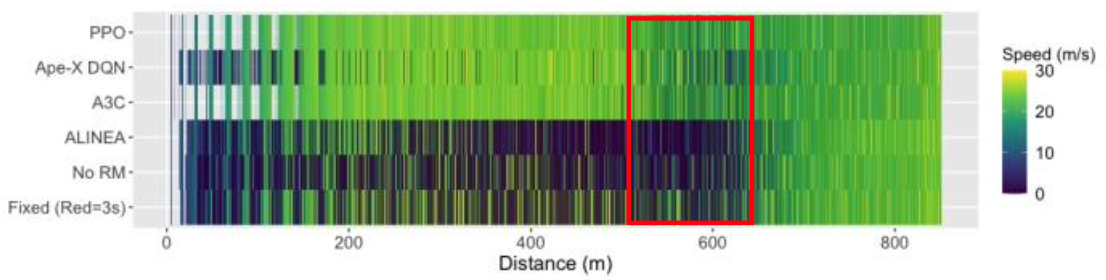
\includegraphics[width=\linewidth]{figures/results/Tuned/Mixed/speedmap_mixed_original.png}
  \end{minipage}
  \hfill
  \begin{minipage}[t]{0.48\linewidth}
    \centering
    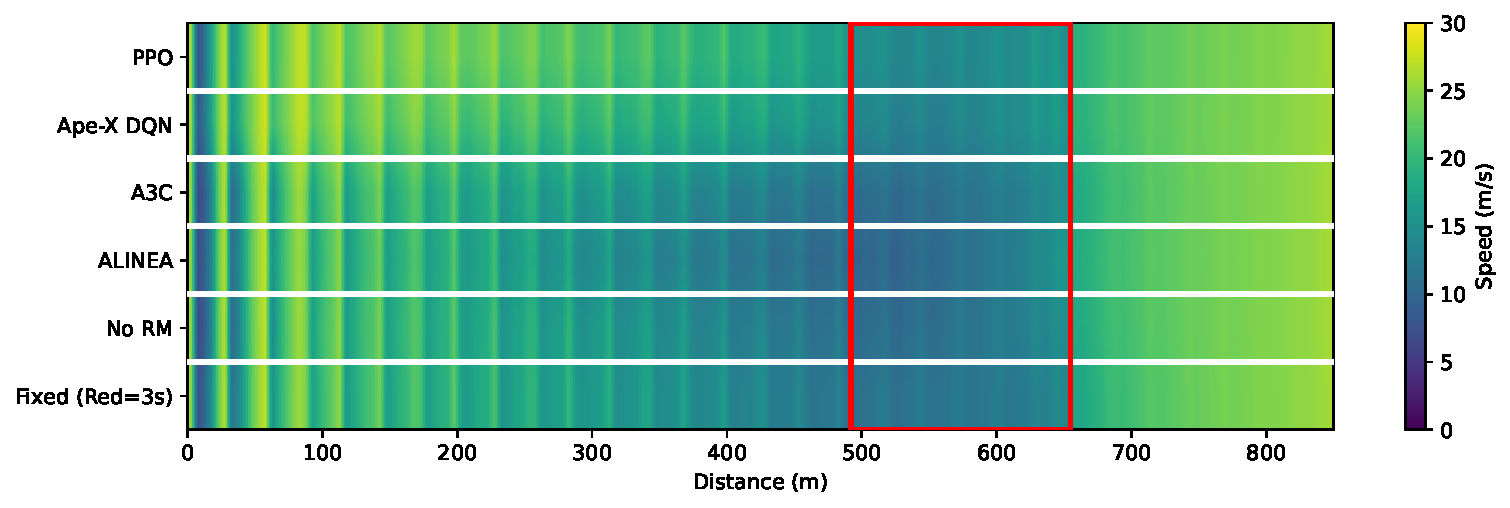
\includegraphics[width=\linewidth]{figures/results/Default/mixed/figure6_mixed.pdf}
  \end{minipage}
  \caption{Spatial speed distribution for the mixed traffic scenario (default setup): original (left) vs.\ replication (right).}
\end{figure}

\begin{figure}[H]
  \centering
  \begin{minipage}[t]{0.48\linewidth}
    \centering
    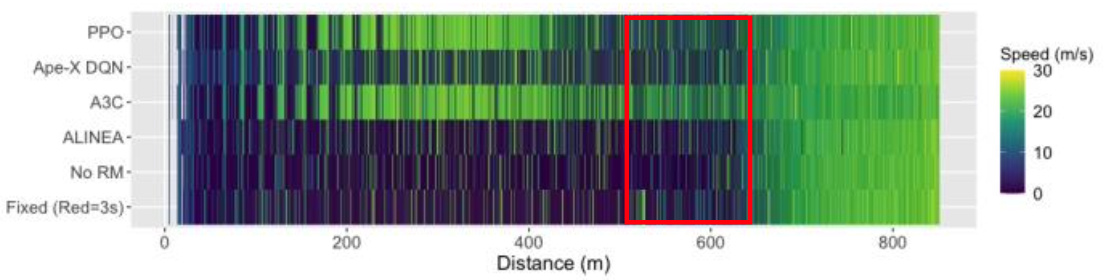
\includegraphics[width=\linewidth]{figures/results/Tuned/Extreme/speedmap_extreme_original.png}
  \end{minipage}
  \hfill
  \begin{minipage}[t]{0.48\linewidth}
    \centering
    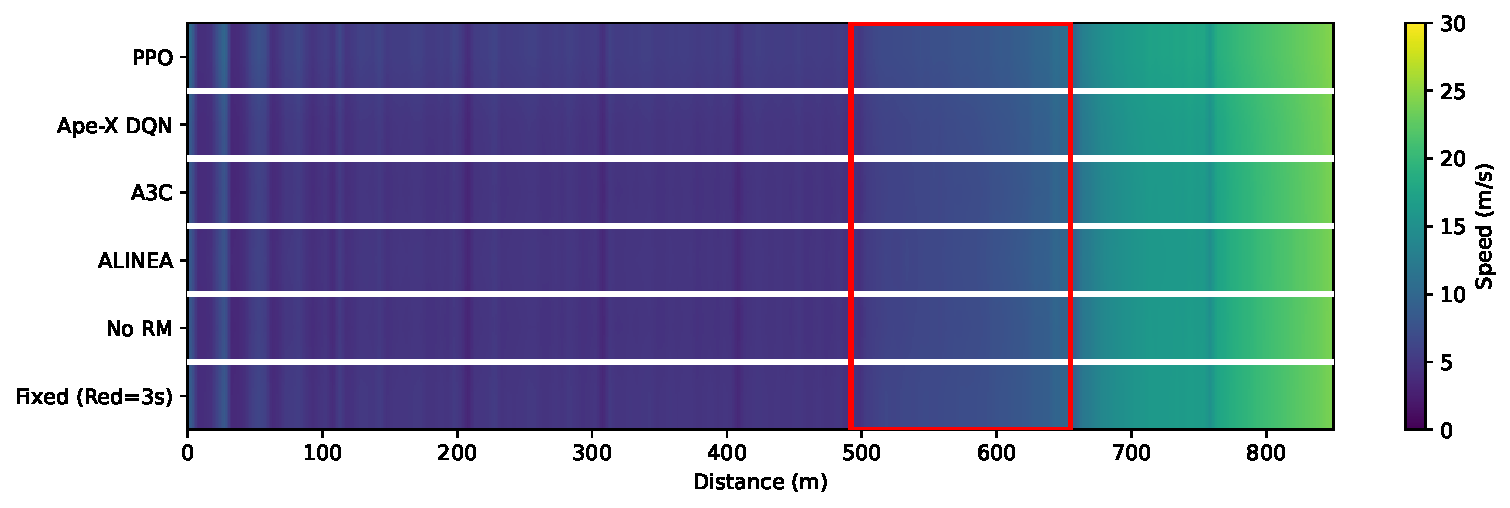
\includegraphics[width=\linewidth]{figures/results/Default/extreme/figure6_extreme.pdf}
  \end{minipage}
  \caption{Spatial speed distribution for the extreme traffic scenario (default setup): original (left) vs.\ replication (right).}
\end{figure}
